\subsection{Vehicle Core Systems}
\subsubsection{Mechanical System}

\paragraph{Frame} \ \\
\vspace{-0.5cm}

Kamikaze’s frame (Figure \ref{fig:frame}) is designed using a cuboid aluminum V-extrusion structure, providing a stable and modular foundation for mounting various components. The 20×20 and 20×40 aluminum extrusions offer a strong yet lightweight framework that maintains structural integrity in underwater conditions.

\hspace{10pt} To enhance stability and buoyancy, HDPE side frame sheets (Figure \ref{fig:side_frame}) are integrated into the design. These sheets not only contribute to the aesthetic appeal of the ROV but also help in maintaining balance during operations. Their strategic placement ensures that the ROV remains hydrodynamically stable while supporting the overall structural framework.

\hspace{10pt} The frame is designed with precise mounting slots, allowing secure positioning of thrusters, cameras, and operational tools while maintaining easy access for maintenance. The bolted assembly ensures that components can be reconfigured or replaced without permanent modifications.

\hspace{10pt} Additionally, the frame is tailored for the E-JUST Robotics team, ensuring compatibility with the mission requirements of the MATE ROV competition while balancing durability, weight efficiency, and adaptability.

\begin{figure}[b]
    \centering
    \begin{subfigure}[b]{0.45\columnwidth}
        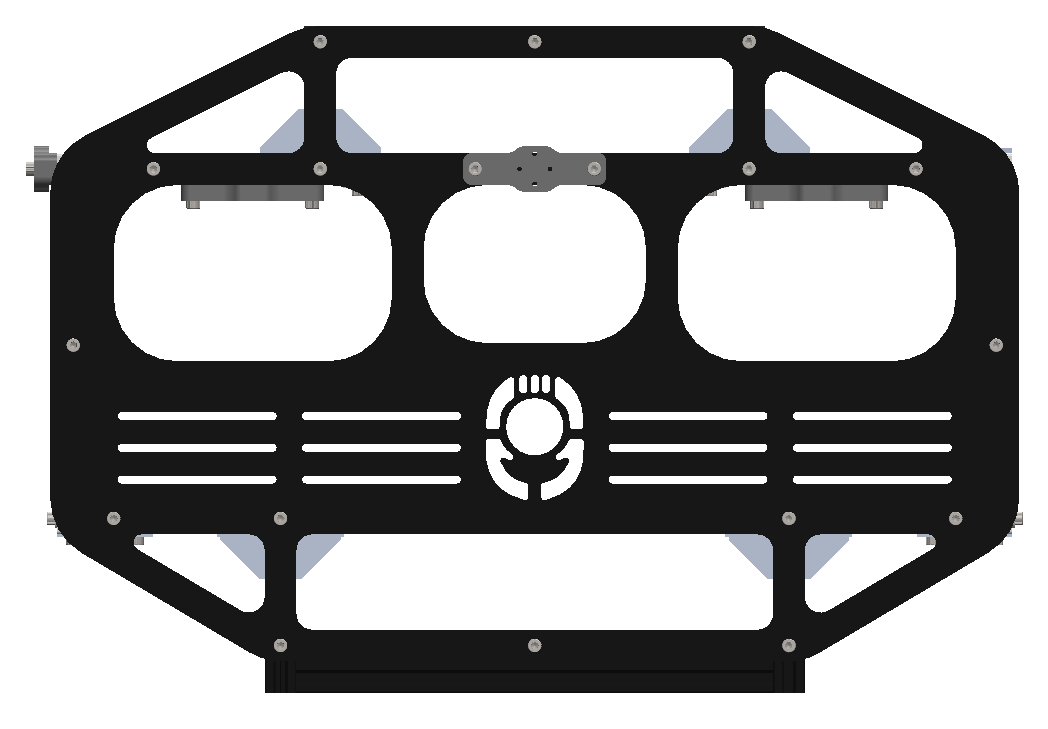
\includegraphics[width=\textwidth]{Sections/2Design Rationale/images/side frame.png}
        \caption{HDPE Side Frame.}
        \label{fig:side_frame}
    \end{subfigure}
    \hfill
    \begin{subfigure}[b]{0.5\columnwidth}
        \includegraphics[width=\textwidth]{Sections/2Design Rationale/images/frame.png}
        \caption{Aluminum Extrusion Frame.}
        \label{fig:frame}
    \end{subfigure}
    \caption{Kamikaze's Frame Illustration.}
    \label{fig:full_frame}
\end{figure}

\vspace{-0.3cm}
\paragraph{Propulsion} \ \\
\vspace{-0.5cm}

Kamikaze is equipped with seven T200 Blue Robotics thrusters, strategically placed to achieve six degrees of freedom for precise maneuverability (Figure \ref{fig:dof}). This setup balances performance, power consumption, and cost-efficiency, ensuring mission success without excessive energy use.

\hspace{10pt} Using seven thrusters instead of a larger number reduces power draw while maintaining stability and control. Each thruster's power consumption is affected by drag force, given by:

\begin{equation}
    F_d = \frac{1}{2} C_d \rho A v^2
    \label{eq:drag_force}
\end{equation}

Where:

\vspace{-0.5\baselineskip}
\begin{itemize}
    \setlength{\itemsep}{0pt}
    \item \(F_d\) = Drag force (N)
    \item \(C_d\) = Drag coefficient (ROV shape-dependent)
    \item \(\rho\) = Water density (kg/m\(^3\))
    \item \(A\) = Cross-sectional area (m\(^2\))
    \item \(v\) = ROV velocity (m/s)
\end{itemize}

\begin{figure}[h]
    \centering
    \includegraphics[width=\columnwidth]{Sections/2Design Rationale/images/dof.png}
    \caption{Kamikaze’s Degrees of Freedom.}
    \label{fig:dof}
\end{figure}

A CFD flow simulation was conducted to analyze water flow around Kamikaze (Figure \ref{fig:cfd}), minimizing drag and enhancing hydrodynamic efficiency.

\begin{figure}[h]
    \centering
    \rule{0.8\columnwidth}{4cm}
    \caption{Flow Simulation.}
    \label{fig:cfd}
\end{figure}

\vspace{0.2cm}
\textbf{Trade-offs in Thruster Selection}
\vspace{-0.5\baselineskip}
\begin{itemize}
    \setlength{\itemsep}{0pt}
    \item \textbf{Power vs. Performance:} More thrusters improve stability but increase power consumption. Seven thrusters provide a balance between efficiency and control.
    \item \textbf{Cost vs. Mission Needs:} Reusing last year’s T200 thrusters reduces costs while still meeting competition requirements.
\end{itemize}

\vspace{-0.3cm}
\paragraph{Buoyancy and Stability} \ \\
\vspace{-0.5cm}

The ROV is designed to have positive buoyancy by carefully selecting lightweight materials and ensuring the buoyant force is slightly greater than its weight. Using Archimedes' principle (Equation \ref{eq:buoyancy}) and SolidWorks simulations (Figure \ref{fig:solidworks_buoyancy}), we confirmed that the ROV naturally surfaces while maintaining stability.

\vspace{-1cm}
\begin{equation}
    \label{eq:buoyancy}
    F_B = \rho_{\text{water}} \times \text{Volume Displaced} \times \text{Gravity}
\end{equation}

\vspace{-0.5cm}
\begin{figure}[h]
    \centering
    \begin{subfigure}[t]{0.49\columnwidth}
        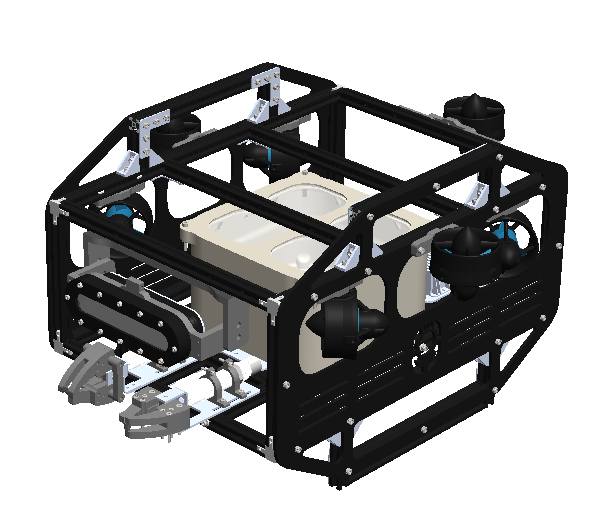
\includegraphics[width=\textwidth]{Sections/2Design Rationale/images/kamikaze_model.png}
        \caption{If an ROV displaces more water than its weight, it floats; otherwise, it sinks.}
        \label{fig:kamikaze}
    \end{subfigure}
    \hfill
    \begin{subfigure}[t]{0.49\columnwidth}
        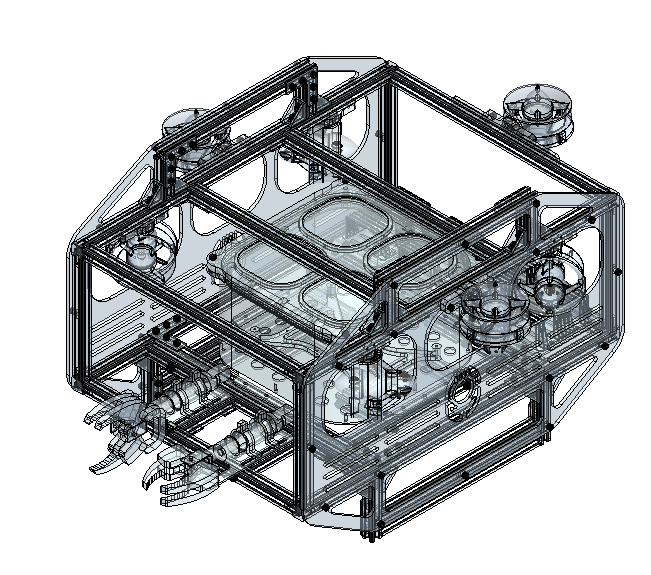
\includegraphics[width=\textwidth]{Sections/2Design Rationale/images/solidworks_buoyancy.png}
        \caption{Buoyancy model in SolidWorks.}
        \label{fig:kamikaze_buoyancy}
    \end{subfigure}
    \caption{SolidWorks analysis for Kamikaze's Buoyancy.}
    \label{fig:solidworks_buoyancy}
\end{figure}

\vspace{-0.3cm}

This was achieved by positioning the center of buoyancy (Table \ref{tab:buoyancy}) above the center of gravity (Table \ref{tab:gravity}), ensuring smooth and controlled movement in the water.

\vspace{-0.7cm}
\begin{center}
\begin{adjustbox}{width=\columnwidth}
    \begin{minipage}[t]{0.48\columnwidth}
    \centering
    \begin{adjustbox}{width=\textwidth, height=0.8cm}
    \renewcommand{\arraystretch}{1.2}
    \begin{tabular}{|l|l|}
    \hline
    \textbf{Parameter} & \textbf{Value} \\
    \hline
    Mass & 18390.88 grams \\
    Volume & 18390882.63 mm\textsuperscript{3} \\
    Center of Buoyancy & X=-0.05, Y=-20.00, Z=-0.10 mm \\
    \hline
    \end{tabular}
    \end{adjustbox}
    \renewcommand{\captionfont}{\footnotesize}
    \captionof{table}{Mass properties of water displaced (buoyancy force)}
    \renewcommand{\captionfont}{\normalsize}
    \label{tab:buoyancy}
    \end{minipage}
    \hfill
    \begin{minipage}[t]{0.48\columnwidth}
    \centering
    \begin{adjustbox}{width=\textwidth, height=0.8cm}
    \renewcommand{\arraystretch}{1.2}
    \begin{tabular}{|l|l|}
    \hline
    \textbf{Parameter} & \textbf{Value} \\
    \hline
    Mass & 17389.17 grams \\
    Volume & 8925547.20 mm\textsuperscript{3} \\
    Center of Gravity & X=0.03, Y=-21.53, Z=-7.36 mm \\
    \hline
    \end{tabular}
    \end{adjustbox}
    \renewcommand{\captionfont}{\footnotesize}
    \captionof{table}{Mass properties of the product and internal components (weight force)}
    \renewcommand{\captionfont}{\normalsize}
    \label{tab:gravity}
    \end{minipage}
\end{adjustbox}
\end{center}

Wet weight is calculated as follows:
\vspace{-0.7\baselineskip}
\[
\begin{aligned}
    Wet \, Weight &= Buoyancy \, Force - Weight \, Force \\
    &= 18,390.88 \, grams - 17,389.17 \, grams \\
    &= 1,001.71 \, grams
\end{aligned}
\]

The buoyancy analysis determined that the ROV, with a mass of 18,390.88 grams, displaces 17,389.17 grams of water, resulting in a net wet weight of 1,001.71 grams. Since it is positively buoyant, the ROV will float. Therefore, after installing the electrical and other components, the buoyancy was checked again to ensure positive buoyancy was maintained. Based on these values, a flotation system was implemented to provide the ROV with a buoyant force of approximately 45 Newtons.

\vspace{-0.3cm}
\paragraph{Main Canister} \ \\
\vspace{-0.5cm}

The canister serves as the primary enclosure for the ROV, protecting essential components such as microcontrollers, power systems, and sensors while ensuring pressure resistance, corrosion protection, and ease of maintenance. The design consists of a 3D-printed PETG body, an aluminum base, and a PETG lid with embedded acrylic windows, providing structural stability and waterproof integrity under operational conditions.

\begin{figure}[h]
    \centering
    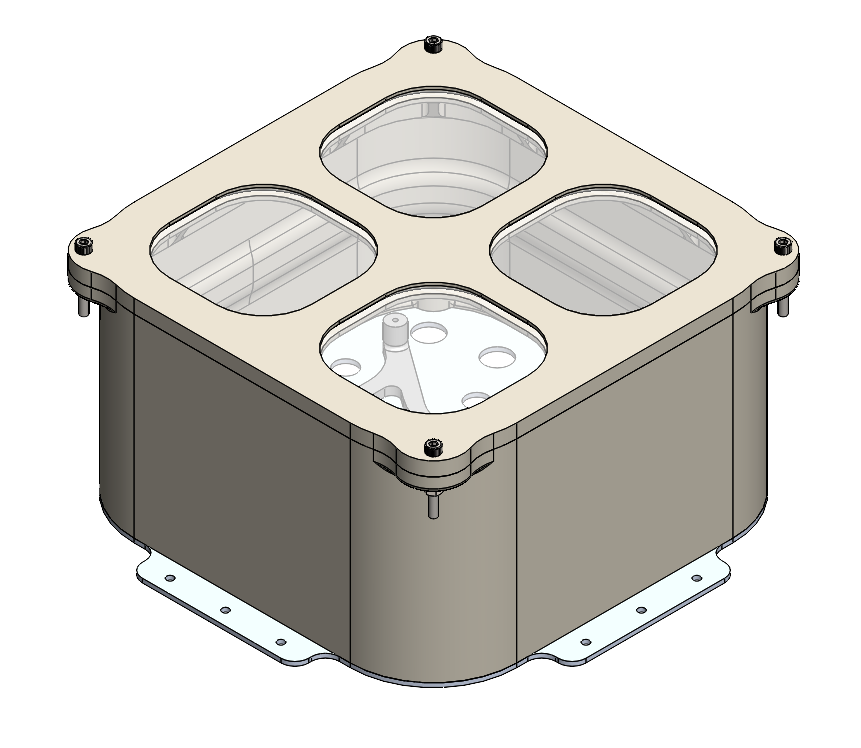
\includegraphics[width=0.6\columnwidth]{Sections/2Design Rationale/images/canister.png}
    \caption{Kamikaze’s Main canister.}
    \label{fig:canister}
\end{figure}

PETG was chosen as a cost-effective alternative to aluminum, offering a balance between mechanical strength and manufacturability. Although PETG is inherently waterproof, Sikadur®-31 CF sealant was applied to enhance structural integrity and reliability. The 3mm-thick aluminum base provides structural support for bulkhead glands, preventing layer separation and ensuring durability. The canister dimensions are 276×276×142.59 mm, optimized for component housing and pressure resistance. A three-stage sealing process was implemented, consisting of mechanical fastening, epoxy bonding, and polyurethane sealant, to maintain a watertight enclosure. The removable PETG lid, secured with M5 screws and dual O-rings, allows for easy inspection and maintenance, while four embedded acrylic windows provide visual access without disassembly.

\hspace{10pt} To evaluate structural performance, a Finite Element Analysis (FEA) was conducted:

\vspace{-0.5\baselineskip}
\begin{itemize}
    \setlength{\itemsep}{0pt}
    \item \textbf{Top View (Figure \ref{fig:top_fda}):} Stress is concentrated around circular openings and edges, which experience higher mechanical loads from water pressure.
    \item \textbf{Bottom View (Figure \ref{fig:bottom_fda}):} Bolted connections and interface zones between the base and side walls accumulate stress, making them susceptible to deformation.
\end{itemize}

\begin{figure}[h]
    \centering
    \begin{subfigure}[b]{0.49\columnwidth}
        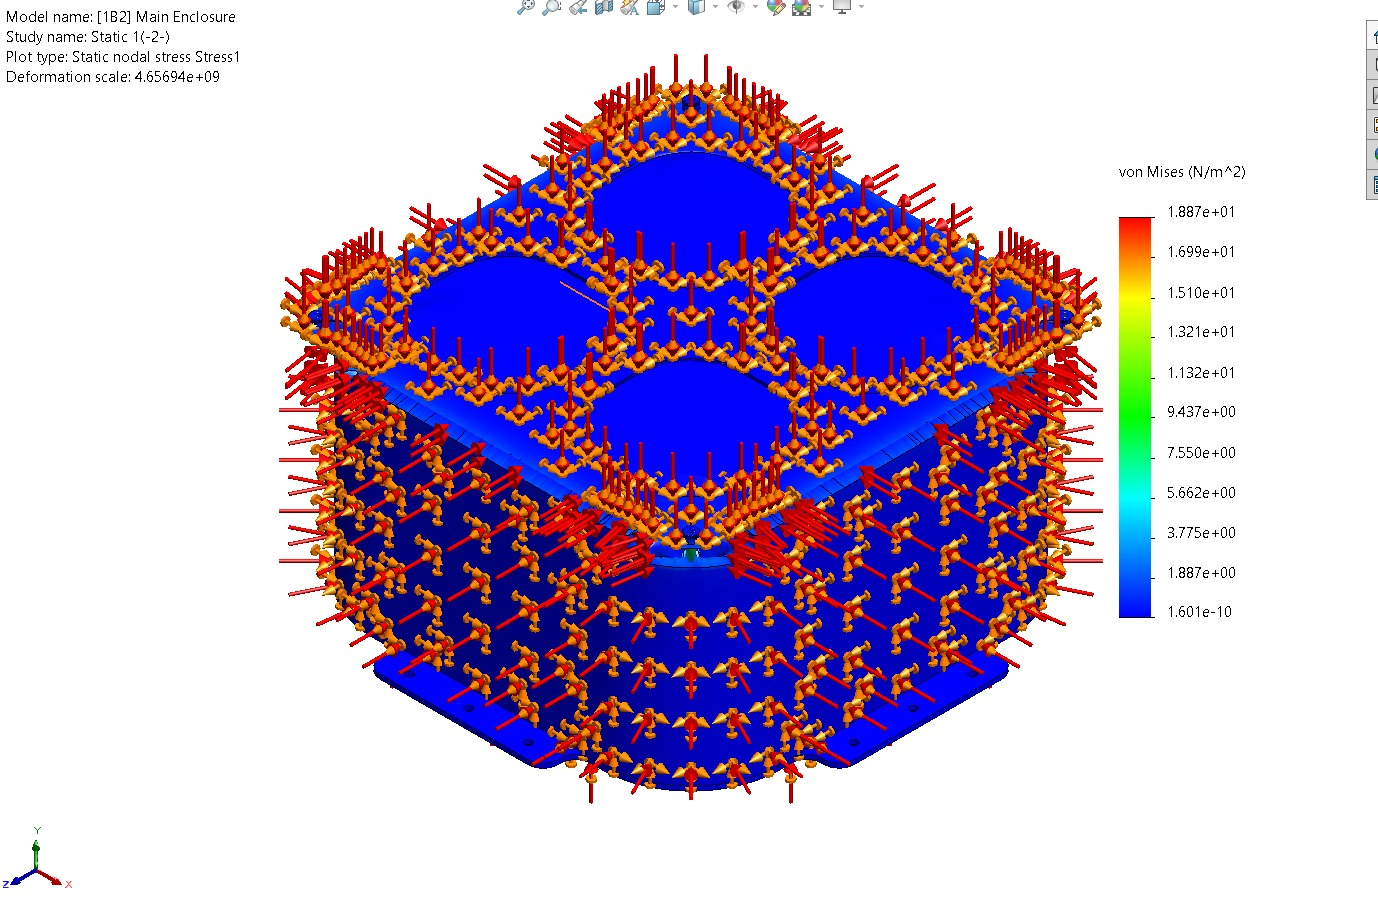
\includegraphics[width=\textwidth]{Sections/2Design Rationale/images/Top view fig stress.jpg}
        \caption{Top View Analysis.}
        \label{fig:top_fda}
    \end{subfigure}
    \hfill
    \begin{subfigure}[b]{0.49\columnwidth}
        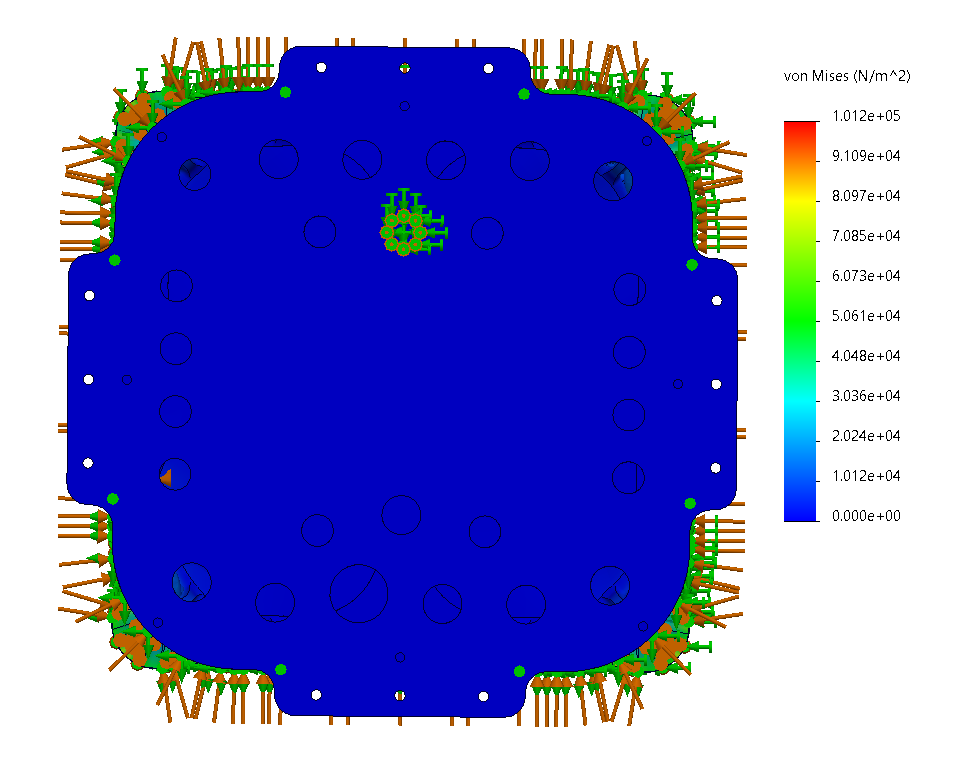
\includegraphics[width=\textwidth]{Sections/2Design Rationale/images/bottom view fig stress.png}
        \caption{Bottom View Analysis.}
        \label{fig:bottom_fda}
    \end{subfigure}
    \caption{Main Canister Finite Element Analysis.}
    \label{fig:fda}
\end{figure}

\vspace{-0.3cm}
\paragraph{Sealing Strategy} \ \\
\vspace{-0.5cm}

Waterproofing is critical for the ROV’s performance and durability. The sealing approach protects electronic components while maintaining structural integrity under varying pressures. This design integrates 3D-printed PETG, aluminum, high-performance adhesives, and mechanical fasteners for optimal sealing efficiency.

\vspace{0.2cm}
\textbf{Main Canister Sealing (Electronics Housing)}

\vspace{-0.5\baselineskip}
\begin{itemize}
    \setlength{\itemsep}{0pt}
    \item Sikadur-31 CF adhesive prevents micro-gaps.
    \item IP68-rated metallic cable glands ensure watertight cable entry.
    \item Epoxy resin \& super glue reinforce adhesion.
    \item Bolted fastening ensures long-term stability.
\end{itemize}

\break

\textbf{ZED Camera Enclosure}

\vspace{-0.7\baselineskip}
\begin{itemize}
    \setlength{\itemsep}{0pt}
    \item O-ring in a groove forms a primary seal.
    \item RTV Gasket Maker provides additional waterproofing.
    \item Compression sealing \& Allen bolts apply uniform pressure.
    \item Sikadur-31 CF protects against water exposure.
    
\end{itemize}

\textbf{Artelon Camera Enclosures}

For other cameras, Artelon enclosures replace aluminum.

\vspace{-0.7\baselineskip}
\begin{itemize}
    \setlength{\itemsep}{0pt}
    \item Acrylic cover sandwiched with an O-ring seal ensures water resistance.
    \item Allen bolts provide tight compression for long-term sealing.
\end{itemize}

\textbf{Bolt Spacing Calculation for Optimal Sealing}

To ensure optimal sealing pressure and prevent gasket deformation under load, the bolt spacing (C) is calculated based on flange stiffness, gasket pressure, and deflection using equation \ref{eq:bolt_spacing}.

\begin{equation} \label{eq:bolt_spacing}
    C = \left[ \frac{480 \left( \frac{a}{b} \right) E t^3 \Delta H}{13 P_{\text{min}} + 2 P_{\text{max}}} \right]^{1/4}
    \end{equation}
    where:
    \vspace{-0.5\baselineskip}
    \begin{itemize}
        \setlength{\itemsep}{0pt}
        \item \(C\) = Bolt spacing (mm)
        \item \(a\) = Width of the flange plate (mm)
        \item \(b\) = Width of the gasket (mm)
        \item \(E\) = Modulus of elasticity of the flange material (Pa or N/m\(^2\))
        \item \(t\) = Thickness of the flange (mm)
        \item \(\Delta H\) = Max. gasket deflection - Min. gasket deflection (mm)
        \item \(P_{\text{min}}\) = Minimum gasket pressure (Pa or N/m\(^2\))
        \item \(P_{\text{max}}\) = Maximum gasket pressure (Pa or N/m\(^2\))
    \end{itemize}
    

\vspace{-0.3cm}
\paragraph{Cameras} \ \\
\vspace{-0.5cm}

To ensure comprehensive underwater vision and precise control of the ROV during operation, a total of six cameras have been integrated into the system. Among these, a ZED camera is strategically placed at the front of the ROV to provide stereoscopic 3D depth perception. The remaining five cameras are a mix of Webcams, Rapoo, and Life Cams, each selected for their reliability, compactness, and clarity in underwater environments. These are distributed across different key positions of the ROV as illustrated in Figure \ref{fig:cameras_enclosures}, ensuring full visual coverage around the vehicle. Their placement allows the pilot to monitor the surroundings of the ROV, including the side and rear views, the grippers, and other mission-specific components.

\begin{figure}[h]
    \centering
    \begin{subfigure}[b]{0.45\columnwidth}
        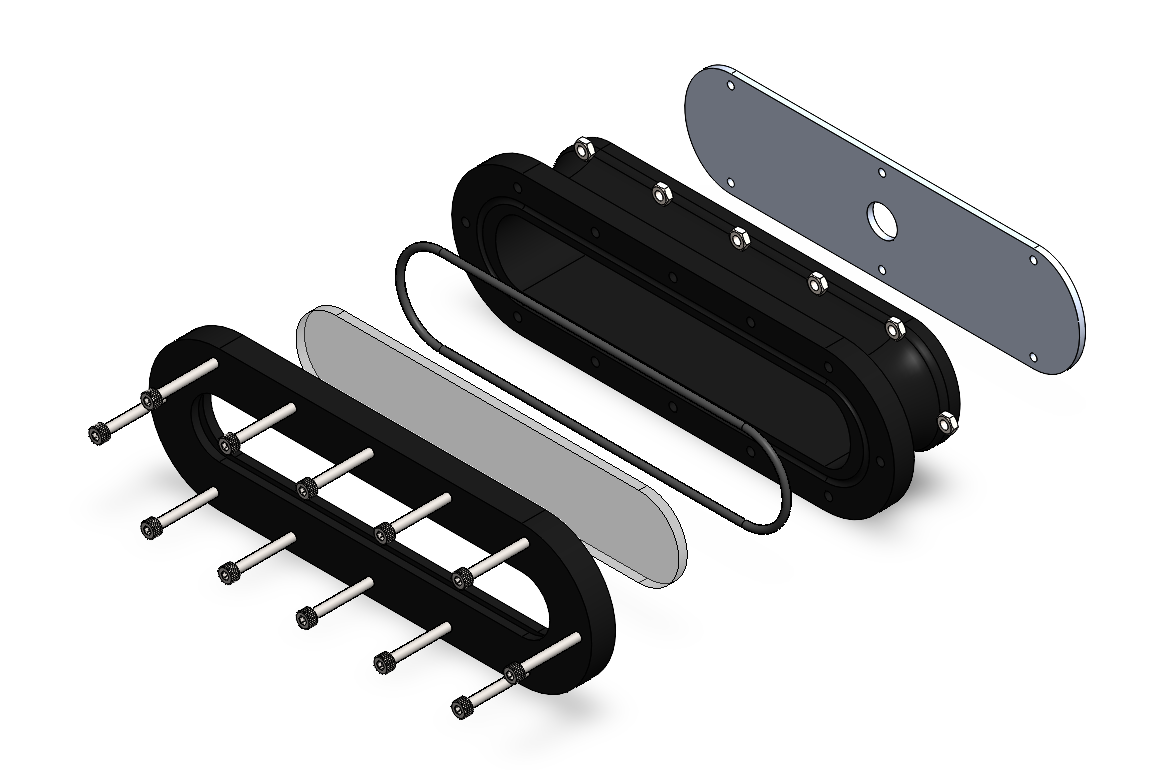
\includegraphics[width=\textwidth]{Sections/2Design Rationale/images/ZED.png}
        \caption{ZED Camera.}
        \label{fig:zed_camera_enclosure}
    \end{subfigure}
    \hfill
    \begin{subfigure}[b]{0.5\columnwidth}
        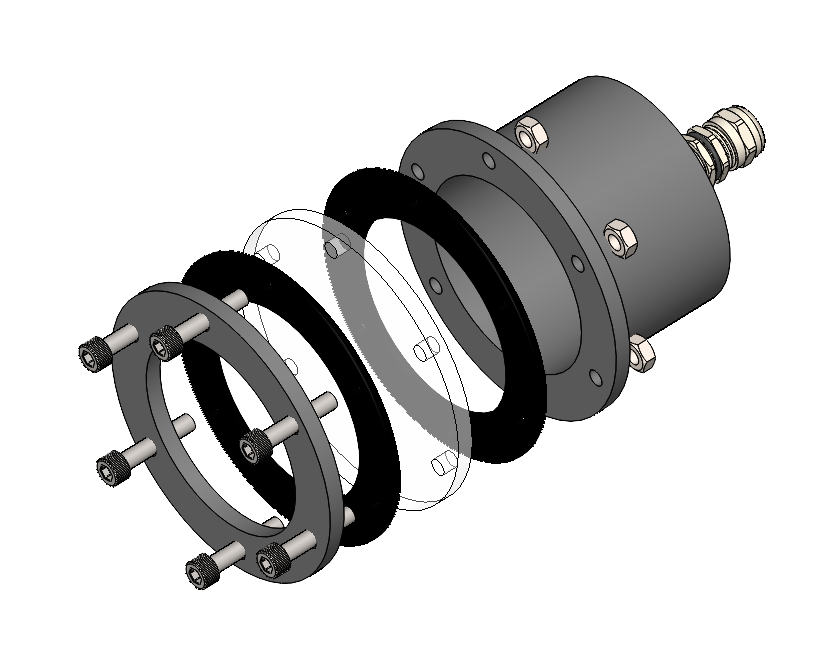
\includegraphics[width=\textwidth]{Sections/2Design Rationale/images/Cameras.png}
        \caption{Other Cameras.}
        \label{fig:other_cameras_enclosure}
    \end{subfigure}
    \caption{Cameras Enclosures.}
    \label{fig:cameras_enclosures}
\end{figure}

\vspace{-0.3cm}
\paragraph{Grippers} \ \\
\vspace{-0.5cm}

Two claw grippers (Figure \ref{fig:grippers}) are designed to handle various item shapes and diameters. They are constructed from 10mm HDPE for durability and aluminum for fixation, ensuring a lightweight yet sturdy design. The grippers are pneumatically actuated using a 25mm stroke piston that applies 113–135N of force in both forward and backward directions. With a maximum opening width of 70mm, they can securely grip all required competition objects. The fluid SID can be found in Appendix \ref{app:fluid_sid}.

\begin{figure}[h]
    \centering
    \begin{subfigure}[b]{0.49\columnwidth}
        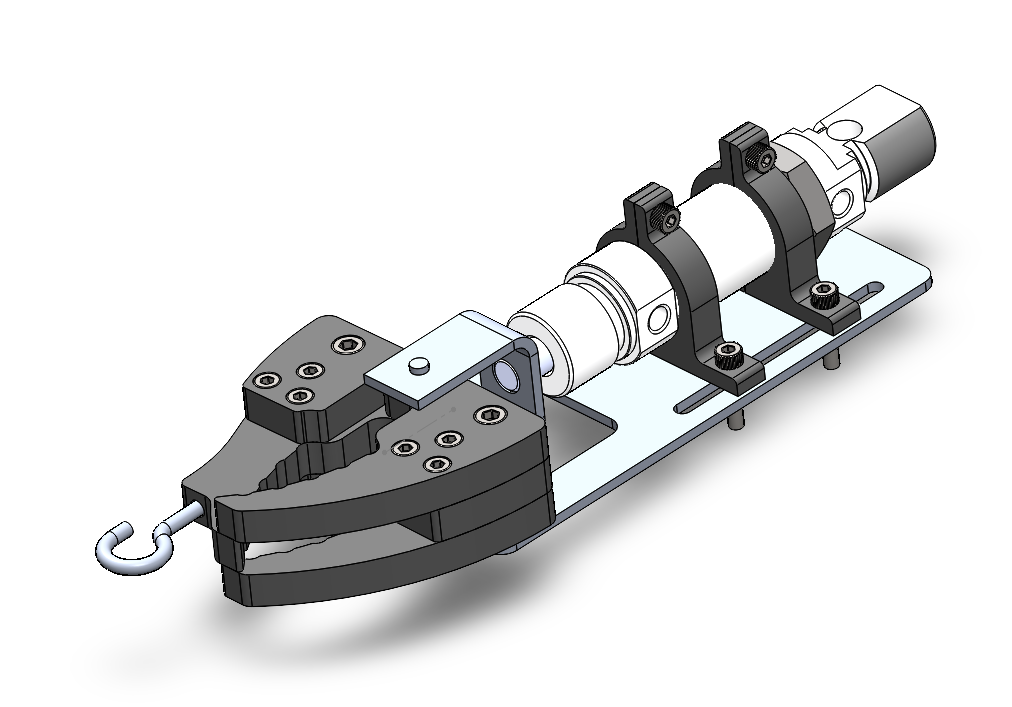
\includegraphics[width=\textwidth]{Sections/2Design Rationale/images/Horizontal.png}
        \caption{Horizontal Gripper.}
        \label{fig:horizontal_gripper}
    \end{subfigure}
    \hfill
    \begin{subfigure}[b]{0.49\columnwidth}
        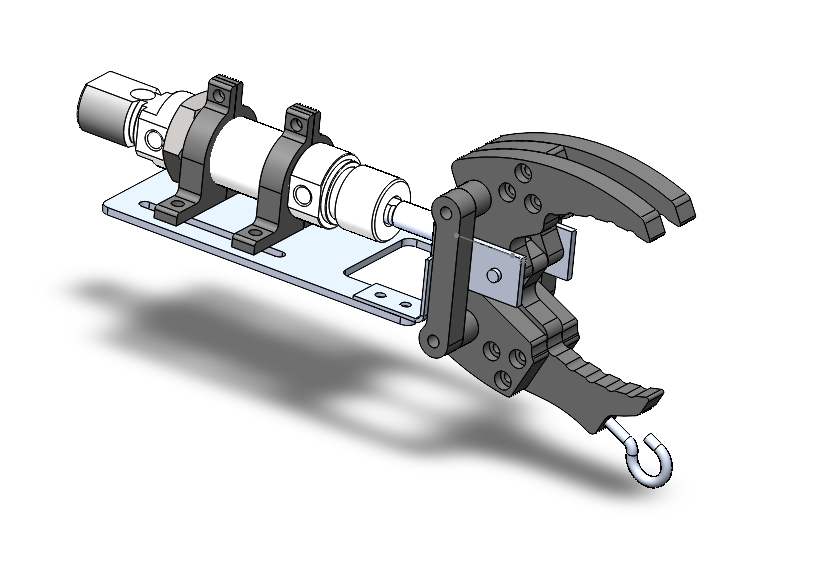
\includegraphics[width=\textwidth]{Sections/2Design Rationale/images/Vertical.png}
        \caption{Vertical Gripper.}
        \label{fig:vertical_gripper}
    \end{subfigure}
    \caption{Kamikaze Grippers.}
    \label{fig:grippers}
\end{figure}

To enhance functionality, two screw hooks were integrated, enabling the ROV to lift hooks and manipulate ropes, expanding its operational capabilities. To optimize the gripper’s design and prevent potential bending stress-induced failures, a comprehensive stress analysis was performed. This theoretical evaluation ensured the gripper’s ability to withstand the designated weight. The results (Figure \ref{fig:grippers_analysis}) confirmed that:

\vspace{-0.5\baselineskip}
\begin{itemize}
    \setlength{\itemsep}{0pt}
    \item The horizontal gripper can hold up to 14.6 kg.
    \item The vertical gripper can hold up to 11.8 kg.
    \item Both with a safety factor of 2.
\end{itemize}

\begin{figure}[h]
    \centering
    \begin{subfigure}[b]{0.49\columnwidth}
        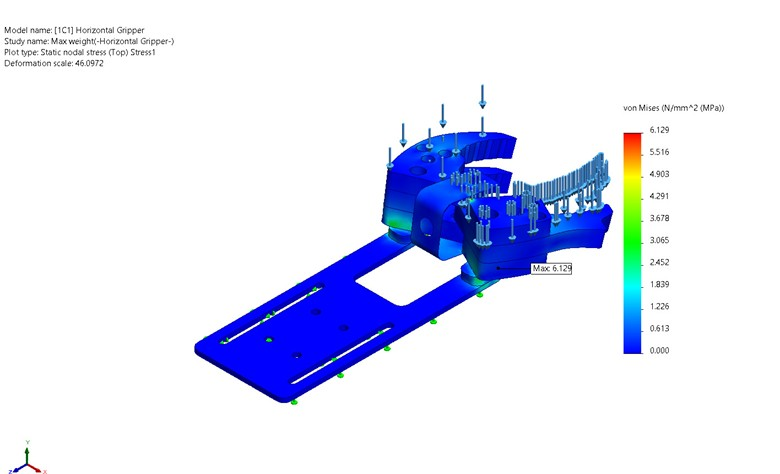
\includegraphics[width=\textwidth]{Sections/2Design Rationale/images/Horizontal Max weight.jpg}
        \caption{Horizontal Gripper Analysis.}
        \label{fig:horizontal_gripper_max_weight}
    \end{subfigure}
    \hfill
    \begin{subfigure}[b]{0.49\columnwidth}
        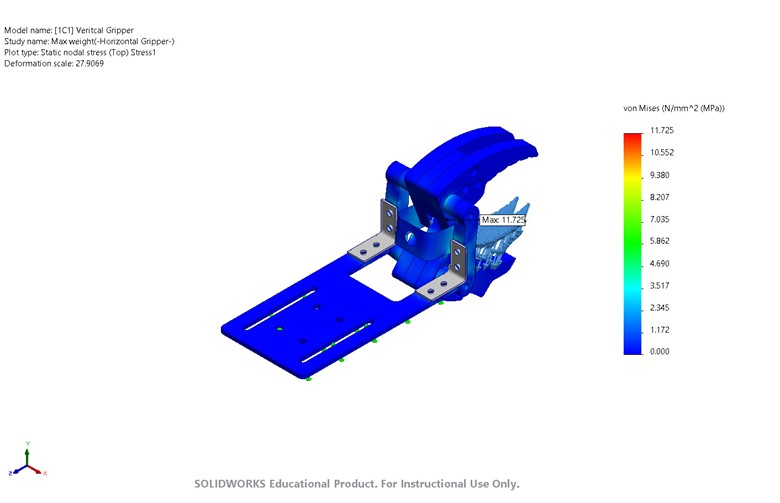
\includegraphics[width=\textwidth]{Sections/2Design Rationale/images/Vertical max weight.jpg}
        \caption{Vertical Gripper Analysis.}
        \label{fig:vertical_gripper_max_weight}
    \end{subfigure}
    \caption{Kamikaze Grippers Analysis.}
    \label{fig:grippers_analysis}
\end{figure}